\scanpage{60}

Bruxelles 5, le 17 octobre 1966\\

Cher Grothendieck,\\

J'ai bien reçu ta lettre.

Je n'ai pas l'intention d'essayer de démontrer, cette année, le ``théorème de \unsure{Lefschetz|Lefchetz} vache''. J'espère donc que tu trouves quelqu'un qui le fasse.

J'ai été malade au début du mois et, comme lecture de convalescence, je lis EGA $\overline{\underline{\mathrm{IV}}}$. Je ne sais pas si tu collectionnes déjà les \unsure{erratas|errata} et compléments pour EGA $0_{\overline{\underline{\mathrm{IV}}}}$ ; je t'envoie toujours ceux qui suivent.

$0_{\overline{\underline{\mathrm{IV}}}}$\quad 19.3.12

\margin{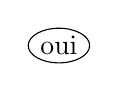
\begin{tikzpicture}[baseline=(n.base)]\node[inner sep=2pt](n){oui};\draw (n.center) ellipse (.39cm and .22cm);\end{tikzpicture}}

est \uuline{canulé} : il faut prendre pour $W_{\unsure{\lambda|s}}$ l'ensemble des homomorphismes d'\uline{algèbre} $B\longrightarrow C_\lambda$ qui relèvent $B\longrightarrow C_\lambda/J_\lambda$, et ce n'est pas une variété linéaire [on n'a pas $J_\lambda^2=0$] - Pour faire marcher l'argument, il faudrait savoir que pour $A$ artinien, l'ensemble des parties de $A^I$ définie par \deleted{\unsure{un syst.}} des équations $P(x_i)\in b$ ($b$ idéal) jouit d'une propriété de compacité. C'est faux pour $I$ infini, déjà pour $A$ un corps infini [$I=k\cup\{\infty\}$, parties $(x_\infty-u)y_u=1$, les $\cap$ finies sont non vides, l'$\cap$ est vide ] - Je crois qu'il n'y a pas d'espoir.

$0_{\overline{\underline{\mathrm{IV}}}}$\quad 17.3.4

Je te signale une jolie démonstration cohomologique de ce résultat, qui fournit un résultat plus complet (lequel se trouve dans Northcott)

\margin{(Th. de Auslander)}

\uline{prop} : $A$ \uline{local noethérien}, $M$ de type fini sur $A$, non nul, et de \uuline{dimension projective finie}. Alors $\underline{\dim\operatorname{proj}(M)=\operatorname{prof} A-\operatorname{prof} M}$.

On utilise la formule suivante, valable pour un complexe parfait $L$ .

\[
\operatorname{RHom}(K,L)=\operatorname{RHom}(K,A)\overset{L}{\otimes}L
\]

avec $K=k$, $L=M$. On trouve une suite spectrale

\[
E_2^{pq}=\operatorname{Tor}_{-p}(\deleted{\unsure{\operatorname{Tor}}}\operatorname{Ext}^{q}(k,A),M)\Longrightarrow \operatorname{Ext}^{p+q}(k,M).\qquad \text{(dessin ci contre)}
\]

\figure{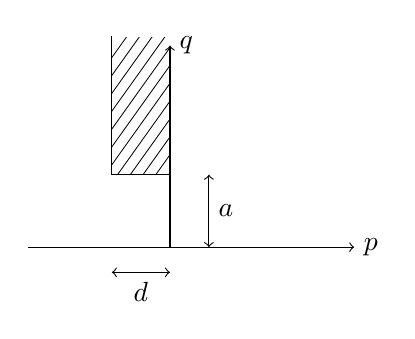
\begin{tikzpicture}[x=0.9cm,y=0.8cm]
\draw[->] (-2,0)--(2.6,0) node[right] {$p$};
\draw[->] (0,0)--(0,3.2) node[right] {$q$};
\draw (-.82,3.35)--(-.82,1.15)--(0,1.15);
\begin{scope}\clip (-.82,1.15) rectangle (0,3.32);
\foreach \a in {-2,-1.82,...,0.2} \draw[line width=.3pt] (\a,1.15)--++(1.65,2.6);
\end{scope}
\draw[<->] (-.82,-.4)--(0,-.4) node[midway,below] {$d$};
\draw[<->] (.55,0)--(.55,1.15) node[midway,right] {$a$};
\end{tikzpicture}}

si $d=\dim\operatorname{proj}M$, $a=\operatorname{prof}A$, on trouve

\[
\begin{aligned}
&\operatorname{Ext}^{n}(k,M)=0\quad\text{si }n<a-d\quad\text{et}\\
&\operatorname{Ext}^{a-d}(k,M)=\operatorname{Tor}_d(\operatorname{Ext}^a(k,A),M)\quad\text{, non nul}
\end{aligned}
\]

par hypothèse (car $\operatorname{Ext}^a(k,A)$ est somme de copies de $k$)

D'où la profondeur de $M$ ...
% archive sheet number: 59
